Ce texte porte sur la mod\'elisation de la propagation d'une \'epid\'emie \footnote{d'après IPT Mines-Ponts 2016}.

Le travail sur ces mod\`eles math\'ematiques s'articule autour de trois th\`emes principaux: traitement de base des donn\'ees, simulation num\'erique (par plusieurs types de m\'ethodes), identification des param\`etres intervenant dans les mod\`eles \`a partir de donn\'ees exp\'erimentales. Ce texte présente deux types de simulation numérique dans des parties \textit{ind\'ependantes}.

Dans tout le probl\`eme, on peut utiliser une fonction trait\'ee pr\'ec\'edemment. On suppose que les biblioth\`eques \texttt{numpy} et \texttt{random} ont \'et\'e import\'ees par:
\begin{verbatim}
import numpy as np
import random as rd
\end{verbatim}

\section*{Partie I. Mod\`ele \`a compartiments}
Les mod\`eles compartimentaux sont des mod\`eles d\'eterministes o\`u la population est divis\'ee en plusieurs cat\'egories selon leurs caract\'eristiques et leur \'etat par rapport \`a la maladie. On consid\`ere dans cette partie un mod\`ele \`a quatre compartiments disjoints: sains (S, "susceptibles"), infect\'es (I,"infected"), r\'etablis(R,"recovered", ils sont immunis\'es) et d\'ec\'ed\'es (D,"dead"). Le changement d'\'etat des individus est gouvern\'e par un syst\`eme d'\'equations diff\'erentielles obtenues en supposant que le nombre d'individus nouvellement infect\'es (c'est-\`a-dire le nombre de ceux qui quittent le compartiment S) pendant un intervalle de temps donn\'e est proportionnel au produit du nombre d'individus infect\'es avec le nombre d'individus sains.

En notant $S(t)$, $I(t)$, $R(t)$ et $D(t)$ la fraction de la population appartenant \`a chacune des quatre cat\'egories \`a l'instant $t$, on obtient le syst\`eme:
\begin{equation}\label{eq1}
\left. \begin{aligned}
\frac{d}{dt}S(t) & =  -rS(t)I(t) \\
\frac{d}{dt}I(t) & =  rS(t)I(t)-(a+b)I(t)\\
\frac{d}{dt}R(t) & =  a I(t) \\
\frac{d}{dt}D(t) & =  bI(t)
\end{aligned} \right\}
\end{equation}
avec $r$ le taux de contagion, $a$ le taux de gu\'erison et $b$ le taux de mortalit\'e. On suppose qu'\`a l'instant initial $t=0$, on a 
\[
S(0)=0,95,\; I(0)=0,05 \text{ et } R(0) = D(0) = 0. 
\]

\begin{enumerate}
\item Pr\'eciser un vecteur $X$ et une fonction $f$ (en donnant son domaine de d\'efinition et son expression) tels que le syst\`eme diff\'erentiel (\ref{eq1}) s'\'ecrive sous la forme
$$
\frac{d}{dt}X = f(X)
$$ 
\item Compl\'eter la ligne 4 du code suivant (on pr\'ecise que \texttt{np.array} permet de cr\'eer un tableau \texttt{numpy} \`a partir d'une liste donnant ainsi la possibilit\'e d'utiliser les op\'erateurs alg\'ebriques).
\begin{lstlisting}
def f(X):
	""" Fonction definissant l'equ. differentielle """
	global r,a,b
	# a completer
	
# Parametres
tmax=25.
r=1.
a=0.4
b=0.1
X0=np.array([0.95,0.05,0.,0.])

N=250
dt=tmax/N

t=0
X=X0
tt=[t]
XX=[X]

# Methode d'Euler
for i in range(N):
	t=t+dt
	X=X+dt*f(X)
	tt.append(t)
	XX.append(X)
\end{lstlisting}

\begin{figure}[!t]
\centering
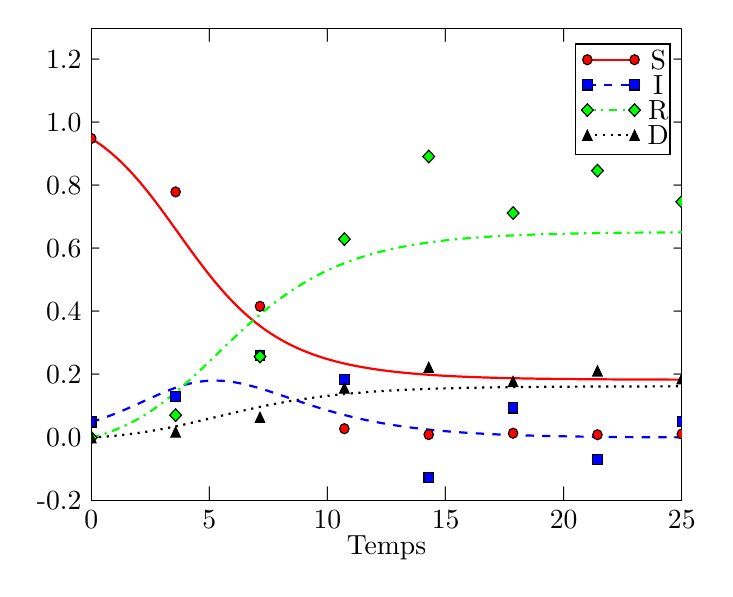
\begin{tikzpicture}[xscale=.3,yscale=4]
\draw (0,-.2) rectangle (25,1.3);
\foreach \n in {0,5,...,25}{
\draw (\n,-.2) node[below]{\n};
}
\foreach \n in {-0.2,0.0,0.2,0.4,0.6,0.8,1.0,1.2}{
\draw (0,\n) node[left]{\n};
}
\draw (12.5,-.28) node[below]{Temps};
\clip (0,-.2) rectangle (25,1.3);
\foreach \n in {5,10,...,20}{
\draw (\n,-.2) node{$|$};
\draw (\n,1.3) node{$|$};
}
\foreach \n in {0.0,0.2,0.4,0.6,0.8,1.0,1.2}{
\draw (0,\n) node{$-$};
\draw (25,\n) node{$-$};
}
\draw[color=red,thick,solid] (0.0,0.95000) -- (0.1,0.94525) -- (0.2,0.94031) -- (0.3,0.93518) -- (0.4,0.92985) -- (0.5,0.92432) -- (0.6,0.91859) -- (0.7,0.91265) -- (0.8,0.90650) -- (0.9,0.90015) -- (1.0,0.89358) -- (1.1,0.88679) -- (1.2,0.87980) -- (1.3,0.87259) -- (1.4,0.86517) -- (1.5,0.85754) -- (1.6,0.84969) -- (1.7,0.84165) -- (1.8,0.83340) -- (1.9,0.82495) -- (2.0,0.81631) -- (2.1,0.80748) -- (2.2,0.79847) -- (2.3,0.78928) -- (2.4,0.77993) -- (2.5,0.77043) -- (2.6,0.76078) -- (2.7,0.75099) -- (2.8,0.74107) -- (2.9,0.73104) -- (3.0,0.72091) -- (3.1,0.71069) -- (3.2,0.70039) -- (3.3,0.69002) -- (3.4,0.67961) -- (3.5,0.66915) -- (3.6,0.65867) -- (3.7,0.64819) -- (3.8,0.63770) -- (3.9,0.62723) -- (4.0,0.61679) -- (4.1,0.60640) -- (4.2,0.59606) -- (4.3,0.58579) -- (4.4,0.57560) -- (4.5,0.56550) -- (4.6,0.55550) -- (4.7,0.54561) -- (4.8,0.53585) -- (4.9,0.52622) -- (5.0,0.51673) -- (5.1,0.50738) -- (5.2,0.49819) -- (5.3,0.48915) -- (5.4,0.48029) -- (5.5,0.47159) -- (5.6,0.46307) -- (5.7,0.45472) -- (5.8,0.44656) -- (5.9,0.43858) -- (6.0,0.43078) -- (6.1,0.42317) -- (6.2,0.41574) -- (6.3,0.40851) -- (6.4,0.40145) -- (6.5,0.39459) -- (6.6,0.38790) -- (6.7,0.38140) -- (6.8,0.37508) -- (6.9,0.36894) -- (7.0,0.36297) -- (7.1,0.35718) -- (7.2,0.35156) -- (7.3,0.34610) -- (7.4,0.34081) -- (7.5,0.33568) -- (7.6,0.33071) -- (7.7,0.32590) -- (7.8,0.32123) -- (7.9,0.31671) -- (8.0,0.31233) -- (8.1,0.30810) -- (8.2,0.30399) -- (8.3,0.30002) -- (8.4,0.29618) -- (8.5,0.29247) -- (8.6,0.28888) -- (8.7,0.28540) -- (8.8,0.28204) -- (8.9,0.27879) -- (9.0,0.27564) -- (9.1,0.27260) -- (9.2,0.26967) -- (9.3,0.26683) -- (9.4,0.26408) -- (9.5,0.26143) -- (9.6,0.25886) -- (9.7,0.25638) -- (9.8,0.25398) -- (9.9,0.25167) -- (10.0,0.24943) -- (10.1,0.24726) -- (10.2,0.24517) -- (10.3,0.24315) -- (10.4,0.24120) -- (10.5,0.23931) -- (10.6,0.23748) -- (10.7,0.23572) -- (10.8,0.23402) -- (10.9,0.23237) -- (11.0,0.23078) -- (11.1,0.22924) -- (11.2,0.22775) -- (11.3,0.22631) -- (11.4,0.22492) -- (11.5,0.22358) -- (11.6,0.22228) -- (11.7,0.22102) -- (11.8,0.21981) -- (11.9,0.21863) -- (12.0,0.21750) -- (12.1,0.21640) -- (12.2,0.21534) -- (12.3,0.21432) -- (12.4,0.21333) -- (12.5,0.21237) -- (12.6,0.21144) -- (12.7,0.21054) -- (12.8,0.20968) -- (12.9,0.20884) -- (13.0,0.20803) -- (13.1,0.20724) -- (13.2,0.20648) -- (13.3,0.20575) -- (13.4,0.20504) -- (13.5,0.20436) -- (13.6,0.20369) -- (13.7,0.20305) -- (13.8,0.20243) -- (13.9,0.20183) -- (14.0,0.20125) -- (14.1,0.20068) -- (14.2,0.20014) -- (14.3,0.19961) -- (14.4,0.19911) -- (14.5,0.19861) -- (14.6,0.19814) -- (14.7,0.19768) -- (14.8,0.19723) -- (14.9,0.19680) -- (15.0,0.19638) -- (15.1,0.19598) -- (15.2,0.19559) -- (15.3,0.19521) -- (15.4,0.19484) -- (15.5,0.19449) -- (15.6,0.19414) -- (15.7,0.19381) -- (15.8,0.19349) -- (15.9,0.19318) -- (16.0,0.19288) -- (16.1,0.19259) -- (16.2,0.19231) -- (16.3,0.19203) -- (16.4,0.19177) -- (16.5,0.19151) -- (16.6,0.19127) -- (16.7,0.19103) -- (16.8,0.19080) -- (16.9,0.19057) -- (17.0,0.19036) -- (17.1,0.19015) -- (17.2,0.18994) -- (17.3,0.18975) -- (17.4,0.18955) -- (17.5,0.18937) -- (17.6,0.18919) -- (17.7,0.18902) -- (17.8,0.18885) -- (17.9,0.18869) -- (18.0,0.18853) -- (18.1,0.18838) -- (18.2,0.18823) -- (18.3,0.18809) -- (18.4,0.18795) -- (18.5,0.18782) -- (18.6,0.18769) -- (18.7,0.18757) -- (18.8,0.18745) -- (18.9,0.18733) -- (19.0,0.18722) -- (19.1,0.18711) -- (19.2,0.18700) -- (19.3,0.18690) -- (19.4,0.18680) -- (19.5,0.18670) -- (19.6,0.18661) -- (19.7,0.18652) -- (19.8,0.18643) -- (19.9,0.18635) -- (20.0,0.18626) -- (20.1,0.18618) -- (20.2,0.18611) -- (20.3,0.18603) -- (20.4,0.18596) -- (20.5,0.18589) -- (20.6,0.18582) -- (20.7,0.18576) -- (20.8,0.18569) -- (20.9,0.18563) -- (21.0,0.18557) -- (21.1,0.18552) -- (21.2,0.18546) -- (21.3,0.18541) -- (21.4,0.18535) -- (21.5,0.18530) -- (21.6,0.18525) -- (21.7,0.18521) -- (21.8,0.18516) -- (21.9,0.18512) -- (22.0,0.18507) -- (22.1,0.18503) -- (22.2,0.18499) -- (22.3,0.18495) -- (22.4,0.18492) -- (22.5,0.18488) -- (22.6,0.18484) -- (22.7,0.18481) -- (22.8,0.18478) -- (22.9,0.18474) -- (23.0,0.18471) -- (23.1,0.
18468) -- (23.2,0.18465) -- (23.3,0.18462) -- (23.4,0.18460) -- (23.5,0.18457) -- (23.6,0.18454) -- (23.7,0.18452) -- (23.8,0.18450) -- (23.9,0.18447) -- (24.0,0.18445) -- (24.1,0.18443) -- (24.2,0.18441) -- (24.3,0.18439) -- (24.4,0.18437) -- (24.5,0.18435) -- (24.6,0.18433) -- (24.7,0.18431) -- (24.8,0.18429) -- (24.9,0.18428) -- (25.0,0.18426);\draw[color=blue,thick,dashed] (0.0,0.05000) -- (0.1,0.05225) -- (0.2,0.05458) -- (0.3,0.05698) -- (0.4,0.05946) -- (0.5,0.06201) -- (0.6,0.06465) -- (0.7,0.06735) -- (0.8,0.07013) -- (0.9,0.07298) -- (1.0,0.07590) -- (1.1,0.07889) -- (1.2,0.08194) -- (1.3,0.08505) -- (1.4,0.08822) -- (1.5,0.09144) -- (1.6,0.09471) -- (1.7,0.09803) -- (1.8,0.10138) -- (1.9,0.10475) -- (2.0,0.10816) -- (2.1,0.11158) -- (2.2,0.11501) -- (2.3,0.11844) -- (2.4,0.12187) -- (2.5,0.12528) -- (2.6,0.12867) -- (2.7,0.13202) -- (2.8,0.13534) -- (2.9,0.13860) -- (3.0,0.14180) -- (3.1,0.14494) -- (3.2,0.14799) -- (3.3,0.15096) -- (3.4,0.15382) -- (3.5,0.15659) -- (3.6,0.15924) -- (3.7,0.16176) -- (3.8,0.16416) -- (3.9,0.16642) -- (4.0,0.16854) -- (4.1,0.17051) -- (4.2,0.17232) -- (4.3,0.17397) -- (4.4,0.17547) -- (4.5,0.17679) -- (4.6,0.17795) -- (4.7,0.17894) -- (4.8,0.17976) -- (4.9,0.18040) -- (5.0,0.18087) -- (5.1,0.18118) -- (5.2,0.18131) -- (5.3,0.18128) -- (5.4,0.18108) -- (5.5,0.18072) -- (5.6,0.18021) -- (5.7,0.17954) -- (5.8,0.17873) -- (5.9,0.17778) -- (6.0,0.17668) -- (6.1,0.17546) -- (6.2,0.17411) -- (6.3,0.17265) -- (6.4,0.17107) -- (6.5,0.16938) -- (6.6,0.16759) -- (6.7,0.16572) -- (6.8,0.16375) -- (6.9,0.16171) -- (7.0,0.15959) -- (7.1,0.15740) -- (7.2,0.15515) -- (7.3,0.15285) -- (7.4,0.15050) -- (7.5,0.14810) -- (7.6,0.14567) -- (7.7,0.14320) -- (7.8,0.14071) -- (7.9,0.13819) -- (8.0,0.13566) -- (8.1,0.13311) -- (8.2,0.13056) -- (8.3,0.12800) -- (8.4,0.12544) -- (8.5,0.12288) -- (8.6,0.12033) -- (8.7,0.11779) -- (8.8,0.11526) -- (8.9,0.11275) -- (9.0,0.11026) -- (9.1,0.10778) -- (9.2,0.10533) -- (9.3,0.10291) -- (9.4,0.10051) -- (9.5,0.09814) -- (9.6,0.09580) -- (9.7,0.09349) -- (9.8,0.09121) -- (9.9,0.08896) -- (10.0,0.08675) -- (10.1,0.08458) -- (10.2,0.08244) -- (10.3,0.08034) -- (10.4,0.07828) -- (10.5,0.07625) -- (10.6,0.07426) -- (10.7,0.07232) -- (10.8,0.07040) -- (10.9,0.06853) -- (11.0,0.06670) -- (11.1,0.06490) -- (11.2,0.06314) -- (11.3,0.06143) -- (11.4,0.05974) -- (11.5,0.05810) -- (11.6,0.05649) -- (11.7,0.05493) -- (11.8,0.05339) -- (11.9,0.05190) -- (12.0,0.05044) -- (12.1,0.04901) -- (12.2,0.04762) -- (12.3,0.04627) -- (12.4,0.04495) -- (12.5,0.04366) -- (12.6,0.04240) -- (12.7,0.04118) -- (12.8,0.03999) -- (12.9,0.03882) -- (13.0,0.03769) -- (13.1,0.03659) -- (13.2,0.03552) -- (13.3,0.03448) -- (13.4,0.03347) -- (13.5,0.03248) -- (13.6,0.03152) -- (13.7,0.03058) -- (13.8,0.02968) -- (13.9,0.02879) -- (14.0,0.02793) -- (14.1,0.02710) -- (14.2,0.02629) -- (14.3,0.02550) -- (14.4,0.02473) -- (14.5,0.02399) -- (14.6,0.02327) -- (14.7,0.02256) -- (14.8,0.02188) -- (14.9,0.02122) -- (15.0,0.02058) -- (15.1,0.01995) -- (15.2,0.01935) -- (15.3,0.01876) -- (15.4,0.01818) -- (15.5,0.01763) -- (15.6,0.01709) -- (15.7,0.01657) -- (15.8,0.01606) -- (15.9,0.01557) -- (16.0,0.01509) -- (16.1,0.01463) -- (16.2,0.01418) -- (16.3,0.01374) -- (16.4,0.01332) -- (16.5,0.01291) -- (16.6,0.01251) -- (16.7,0.01212) -- (16.8,0.01175) -- (16.9,0.01139) -- (17.0,0.01103) -- (17.1,0.01069) -- (17.2,0.01036) -- (17.3,0.01004) -- (17.4,0.00973) -- (17.5,0.00943) -- (17.6,0.00913) -- (17.7,0.00885) -- (17.8,0.00857) -- (17.9,0.00831) -- (18.0,0.00805) -- (18.1,0.00780) -- (18.2,0.00755) -- (18.3,0.00732) -- (18.4,0.00709) -- (18.5,0.00687) -- (18.6,0.00666) -- (18.7,0.00645) -- (18.8,0.00625) -- (18.9,0.00605) -- (19.0,0.00586) -- (19.1,0.00568) -- (19.2,0.00550) -- (19.3,0.00533) -- (19.4,0.00516) -- (19.5,0.00500) -- (19.6,0.00484) -- (19.7,0.00469) -- (19.8,0.00454) -- (19.9,0.00440) -- (20.0,0.00426) -- (20.1,0.00413) -- (20.2,0.00400) -- (20.3,0.00387) -- (20.4,0.00375) -- (20.5,0.00364) -- (20.6,0.00352) -- (20.7,0.00341) -- (20.8,0.00330) -- (20.9,0.00320) -- (21.0,0.00310) -- (21.1,0.00300) -- 
(21.2,0.00291) -- (21.3,0.00282) -- (21.4,0.00273) -- (21.5,0.00264) -- (21.6,0.00256) -- (21.7,0.00248) -- (21.8,0.00240) -- (21.9,0.00232) -- (22.0,0.00225) -- (22.1,0.00218) -- (22.2,0.00211) -- (22.3,0.00204) -- (22.4,0.00198) -- (22.5,0.00192) -- (22.6,0.00186) -- (22.7,0.00180) -- (22.8,0.00174) -- (22.9,0.00169) -- (23.0,0.00163) -- (23.1,0.00158) -- (23.2,0.00153) -- (23.3,0.00148) -- (23.4,0.00144) -- (23.5,0.00139) -- (23.6,0.00135) -- (23.7,0.00131) -- (23.8,0.00126) -- (23.9,0.00122) -- (24.0,0.00119) -- (24.1,0.00115) -- (24.2,0.00111) -- (24.3,0.00108) -- (24.4,0.00104) -- (24.5,0.00101) -- (24.6,0.00098) -- (24.7,0.00095) -- (24.8,0.00092) -- (24.9,0.00089) -- (25.0,0.00086);\draw[color=green,thick,dashdotted] (0.0,0.00000) -- (0.1,0.00200) -- (0.2,0.00409) -- (0.3,0.00627) -- (0.4,0.00855) -- (0.5,0.01093) -- (0.6,0.01341) -- (0.7,0.01600) -- (0.8,0.01869) -- (0.9,0.02150) -- (1.0,0.02442) -- (1.1,0.02745) -- (1.2,0.03061) -- (1.3,0.03389) -- (1.4,0.03729) -- (1.5,0.04082) -- (1.6,0.04447) -- (1.7,0.04826) -- (1.8,0.05218) -- (1.9,0.05624) -- (2.0,0.06043) -- (2.1,0.06476) -- (2.2,0.06922) -- (2.3,0.07382) -- (2.4,0.07856) -- (2.5,0.08343) -- (2.6,0.08844) -- (2.7,0.09359) -- (2.8,0.09887) -- (2.9,0.10428) -- (3.0,0.10983) -- (3.1,0.11550) -- (3.2,0.12130) -- (3.3,0.12722) -- (3.4,0.13326) -- (3.5,0.13941) -- (3.6,0.14567) -- (3.7,0.15204) -- (3.8,0.15851) -- (3.9,0.16508) -- (4.0,0.17173) -- (4.1,0.17848) -- (4.2,0.18530) -- (4.3,0.19219) -- (4.4,0.19915) -- (4.5,0.20617) -- (4.6,0.21324) -- (4.7,0.22036) -- (4.8,0.22751) -- (4.9,0.23470) -- (5.0,0.24192) -- (5.1,0.24916) -- (5.2,0.25640) -- (5.3,0.26365) -- (5.4,0.27091) -- (5.5,0.27815) -- (5.6,0.28538) -- (5.7,0.29259) -- (5.8,0.29977) -- (5.9,0.30692) -- (6.0,0.31403) -- (6.1,0.32110) -- (6.2,0.32811) -- (6.3,0.33508) -- (6.4,0.34198) -- (6.5,0.34883) -- (6.6,0.35560) -- (6.7,0.36231) -- (6.8,0.36893) -- (6.9,0.37548) -- (7.0,0.38195) -- (7.1,0.38834) -- (7.2,0.39463) -- (7.3,0.40084) -- (7.4,0.40695) -- (7.5,0.41297) -- (7.6,0.41890) -- (7.7,0.42472) -- (7.8,0.43045) -- (7.9,0.43608) -- (8.0,0.44161) -- (8.1,0.44703) -- (8.2,0.45236) -- (8.3,0.45758) -- (8.4,0.46270) -- (8.5,0.46772) -- (8.6,0.47263) -- (8.7,0.47745) -- (8.8,0.48216) -- (8.9,0.48677) -- (9.0,0.49128) -- (9.1,0.49569) -- (9.2,0.50000) -- (9.3,0.50421) -- (9.4,0.50833) -- (9.5,0.51235) -- (9.6,0.51628) -- (9.7,0.52011) -- (9.8,0.52385) -- (9.9,0.52750) -- (10.0,0.53105) -- (10.1,0.53452) -- (10.2,0.53791) -- (10.3,0.54121) -- (10.4,0.54442) -- (10.5,0.54755) -- (10.6,0.55060) -- (10.7,0.55357) -- (10.8,0.55646) -- (10.9,0.55928) -- (11.0,0.56202) -- (11.1,0.56469) -- (11.2,0.56728) -- (11.3,0.56981) -- (11.4,0.57227) -- (11.5,0.57466) -- (11.6,0.57698) -- (11.7,0.57924) -- (11.8,0.58144) -- (11.9,0.58357) -- (12.0,0.58565) -- (12.1,0.58767) -- (12.2,0.58963) -- (12.3,0.59153) -- (12.4,0.59338) -- (12.5,0.59518) -- (12.6,0.59693) -- (12.7,0.59862) -- (12.8,0.60027) -- (12.9,0.60187) -- (13.0,0.60342) -- (13.1,0.60493) -- (13.2,0.60639) -- (13.3,0.60782) -- (13.4,0.60919) -- (13.5,0.61053) -- (13.6,0.61183) -- (13.7,0.61309) -- (13.8,0.61432) -- (13.9,0.61550) -- (14.0,0.61666) -- (14.1,0.61777) -- (14.2,0.61886) -- (14.3,0.61991) -- (14.4,0.62093) -- (14.5,0.62192) -- (14.6,0.62288) -- (14.7,0.62381) -- (14.8,0.62471) -- (14.9,0.62559) -- (15.0,0.62643) -- (15.1,0.62726) -- (15.2,0.62806) -- (15.3,0.62883) -- (15.4,0.62958) -- (15.5,0.63031) -- (15.6,0.63101) -- (15.7,0.63170) -- (15.8,0.63236) -- (15.9,0.63300) -- (16.0,0.63362) -- (16.1,0.63423) -- (16.2,0.63481) -- (16.3,0.63538) -- (16.4,0.63593) -- (16.5,0.63646) -- (16.6,0.63698) -- (16.7,0.63748) -- (16.8,0.63796) -- (16.9,0.63843) -- (17.0,0.63889) -- (17.1,0.63933) -- (17.2,0.63976) -- (17.3,0.64017) -- (17.4,0.64057) -- (17.5,0.64096) -- (17.6,0.64134) -- (17.7,0.64171) -- (17.8,0.64206) -- (17.9,0.64240) -- (18.0,0.64273) -- (18.1,0.64306) -- (18.2,0.64337) -- (18.3,0.64367) -- (18.4,0.64396) -- (18.5,0.64425) -- (18.6,0.64452) -- (18.7,0.64479) -- (18.8,0.64505) -- (18.9,0.64530) -- (19.0,0.64554) -- (19.1,0.64577) -- (19.
2,0.64600) -- (19.3,0.64622) -- (19.4,0.64643) -- (19.5,0.64664) -- (19.6,0.64684) -- (19.7,0.64703) -- (19.8,0.64722) -- (19.9,0.64740) -- (20.0,0.64758) -- (20.1,0.64775) -- (20.2,0.64791) -- (20.3,0.64807) -- (20.4,0.64823) -- (20.5,0.64838) -- (20.6,0.64852) -- (20.7,0.64867) -- (20.8,0.64880) -- (20.9,0.64893) -- (21.0,0.64906) -- (21.1,0.64919) -- (21.2,0.64931) -- (21.3,0.64942) -- (21.4,0.64954) -- (21.5,0.64964) -- (21.6,0.64975) -- (21.7,0.64985) -- (21.8,0.64995) -- (21.9,0.65005) -- (22.0,0.65014) -- (22.1,0.65023) -- (22.2,0.65032) -- (22.3,0.65040) -- (22.4,0.65048) -- (22.5,0.65056) -- (22.6,0.65064) -- (22.7,0.65071) -- (22.8,0.65079) -- (22.9,0.65086) -- (23.0,0.65092) -- (23.1,0.65099) -- (23.2,0.65105) -- (23.3,0.65111) -- (23.4,0.65117) -- (23.5,0.65123) -- (23.6,0.65129) -- (23.7,0.65134) -- (23.8,0.65139) -- (23.9,0.65144) -- (24.0,0.65149) -- (24.1,0.65154) -- (24.2,0.65158) -- (24.3,0.65163) -- (24.4,0.65167) -- (24.5,0.65171) -- (24.6,0.65175) -- (24.7,0.65179) -- (24.8,0.65183) -- (24.9,0.65187) -- (25.0,0.65190);\draw[color=black,thick,dotted] (0.0,0.00000) -- (0.1,0.00050) -- (0.2,0.00102) -- (0.3,0.00157) -- (0.4,0.00214) -- (0.5,0.00273) -- (0.6,0.00335) -- (0.7,0.00400) -- (0.8,0.00467) -- (0.9,0.00537) -- (1.0,0.00610) -- (1.1,0.00686) -- (1.2,0.00765) -- (1.3,0.00847) -- (1.4,0.00932) -- (1.5,0.01020) -- (1.6,0.01112) -- (1.7,0.01207) -- (1.8,0.01305) -- (1.9,0.01406) -- (2.0,0.01511) -- (2.1,0.01619) -- (2.2,0.01730) -- (2.3,0.01845) -- (2.4,0.01964) -- (2.5,0.02086) -- (2.6,0.02211) -- (2.7,0.02340) -- (2.8,0.02472) -- (2.9,0.02607) -- (3.0,0.02746) -- (3.1,0.02888) -- (3.2,0.03032) -- (3.3,0.03180) -- (3.4,0.03331) -- (3.5,0.03485) -- (3.6,0.03642) -- (3.7,0.03801) -- (3.8,0.03963) -- (3.9,0.04127) -- (4.0,0.04293) -- (4.1,0.04462) -- (4.2,0.04632) -- (4.3,0.04805) -- (4.4,0.04979) -- (4.5,0.05154) -- (4.6,0.05331) -- (4.7,0.05509) -- (4.8,0.05688) -- (4.9,0.05868) -- (5.0,0.06048) -- (5.1,0.06229) -- (5.2,0.06410) -- (5.3,0.06591) -- (5.4,0.06773) -- (5.5,0.06954) -- (5.6,0.07134) -- (5.7,0.07315) -- (5.8,0.07494) -- (5.9,0.07673) -- (6.0,0.07851) -- (6.1,0.08027) -- (6.2,0.08203) -- (6.3,0.08377) -- (6.4,0.08550) -- (6.5,0.08721) -- (6.6,0.08890) -- (6.7,0.09058) -- (6.8,0.09223) -- (6.9,0.09387) -- (7.0,0.09549) -- (7.1,0.09708) -- (7.2,0.09866) -- (7.3,0.10021) -- (7.4,0.10174) -- (7.5,0.10324) -- (7.6,0.10472) -- (7.7,0.10618) -- (7.8,0.10761) -- (7.9,0.10902) -- (8.0,0.11040) -- (8.1,0.11176) -- (8.2,0.11309) -- (8.3,0.11440) -- (8.4,0.11568) -- (8.5,0.11693) -- (8.6,0.11816) -- (8.7,0.11936) -- (8.8,0.12054) -- (8.9,0.12169) -- (9.0,0.12282) -- (9.1,0.12392) -- (9.2,0.12500) -- (9.3,0.12605) -- (9.4,0.12708) -- (9.5,0.12809) -- (9.6,0.12907) -- (9.7,0.13003) -- (9.8,0.13096) -- (9.9,0.13187) -- (10.0,0.13276) -- (10.1,0.13363) -- (10.2,0.13448) -- (10.3,0.13530) -- (10.4,0.13610) -- (10.5,0.13689) -- (10.6,0.13765) -- (10.7,0.13839) -- (10.8,0.13912) -- (10.9,0.13982) -- (11.0,0.14051) -- (11.1,0.14117) -- (11.2,0.14182) -- (11.3,0.14245) -- (11.4,0.14307) -- (11.5,0.14366) -- (11.6,0.14425) -- (11.7,0.14481) -- (11.8,0.14536) -- (11.9,0.14589) -- (12.0,0.14641) -- (12.1,0.14692) -- (12.2,0.14741) -- (12.3,0.14788) -- (12.4,0.14835) -- (12.5,0.14880) -- (12.6,0.14923) -- (12.7,0.14966) -- (12.8,0.15007) -- (12.9,0.15047) -- (13.0,0.15086) -- (13.1,0.15123) -- (13.2,0.15160) -- (13.3,0.15195) -- (13.4,0.15230) -- (13.5,0.15263) -- (13.6,0.15296) -- (13.7,0.15327) -- (13.8,0.15358) -- (13.9,0.15388) -- (14.0,0.15416) -- (14.1,0.15444) -- (14.2,0.15471) -- (14.3,0.15498) -- (14.4,0.15523) -- (14.5,0.15548) -- (14.6,0.15572) -- (14.7,0.15595) -- (14.8,0.15618) -- (14.9,0.15640) -- (15.0,0.15661) -- (15.1,0.15681) -- (15.2,0.15701) -- (15.3,0.15721) -- (15.4,0.15739) -- (15.5,0.15758) -- (15.6,0.15775) -- (15.7,0.15792) -- (15.8,0.15809) -- (15.9,0.15825) -- (16.0,0.15841) -- (16.1,0.15856) -- (16.2,0.15870) -- (16.3,0.15884) -- (16.4,0.15898) -- (16.5,0.15912) -- (16.6,0.15924) -- (16.7,0.15937) -- (16.8,0.15949) -- (16.9,0.15961) -- (17.0,0.15972) -- (17.1,0.15983) -- (17.2,0.
15994) -- (17.3,0.16004) -- (17.4,0.16014) -- (17.5,0.16024) -- (17.6,0.16034) -- (17.7,0.16043) -- (17.8,0.16051) -- (17.9,0.16060) -- (18.0,0.16068) -- (18.1,0.16076) -- (18.2,0.16084) -- (18.3,0.16092) -- (18.4,0.16099) -- (18.5,0.16106) -- (18.6,0.16113) -- (18.7,0.16120) -- (18.8,0.16126) -- (18.9,0.16132) -- (19.0,0.16138) -- (19.1,0.16144) -- (19.2,0.16150) -- (19.3,0.16155) -- (19.4,0.16161) -- (19.5,0.16166) -- (19.6,0.16171) -- (19.7,0.16176) -- (19.8,0.16181) -- (19.9,0.16185) -- (20.0,0.16189) -- (20.1,0.16194) -- (20.2,0.16198) -- (20.3,0.16202) -- (20.4,0.16206) -- (20.5,0.16209) -- (20.6,0.16213) -- (20.7,0.16217) -- (20.8,0.16220) -- (20.9,0.16223) -- (21.0,0.16227) -- (21.1,0.16230) -- (21.2,0.16233) -- (21.3,0.16236) -- (21.4,0.16238) -- (21.5,0.16241) -- (21.6,0.16244) -- (21.7,0.16246) -- (21.8,0.16249) -- (21.9,0.16251) -- (22.0,0.16254) -- (22.1,0.16256) -- (22.2,0.16258) -- (22.3,0.16260) -- (22.4,0.16262) -- (22.5,0.16264) -- (22.6,0.16266) -- (22.7,0.16268) -- (22.8,0.16270) -- (22.9,0.16271) -- (23.0,0.16273) -- (23.1,0.16275) -- (23.2,0.16276) -- (23.3,0.16278) -- (23.4,0.16279) -- (23.5,0.16281) -- (23.6,0.16282) -- (23.7,0.16283) -- (23.8,0.16285) -- (23.9,0.16286) -- (24.0,0.16287) -- (24.1,0.16288) -- (24.2,0.16290) -- (24.3,0.16291) -- (24.4,0.16292) -- (24.5,0.16293) -- (24.6,0.16294) -- (24.7,0.16295) -- (24.8,0.16296) -- (24.9,0.16297) -- (25.0,0.16298);
\filldraw[fill=red] (0.00000,0.95000) ellipse(0.2cm and 0.016cm) (3.57143,0.78036) ellipse(0.2cm and 0.016cm) (7.14286,0.41705) ellipse(0.2cm and 0.016cm) (10.71429,0.02848) ellipse(0.2cm and 0.016cm) (14.28571,0.00980) ellipse(0.2cm and 0.016cm) (17.85714,0.01420) ellipse(0.2cm and 0.016cm)(21.42857,0.00942) ellipse(0.2cm and 0.016cm)(25.00000,0.01175) ellipse(0.2cm and 0.016cm);
\filldraw[fill=blue] (0.00000,0.05000) + (-.2,-.016) rectangle+ (.2,.016) (3.57143,0.13036) + (-.2,-.016) rectangle+ (.2,.016) (7.14286,0.26088) + (-.2,-.016) rectangle+ (.2,.016) (10.71429,0.18360) + (-.2,-.016) rectangle+ (.2,.016) (14.28571,-0.12558) + (-.2,-.016) rectangle+ (.2,.016) (17.85714,0.09427) + (-.2,-.016) rectangle+ (.2,.016) (21.42857,-0.06929) + (-.2,-.016) rectangle+ (.2,.016) (25.00000,0.05211) + (-.2,-.016) rectangle+ (.2,.016);
\filldraw[fill=green] (0.00000,0.00000) + (.25,0) --+ (0,.02) --+ (-.25,0) -- + (0,-.02) --cycle
(3.57143,0.07143)  + (.25,0) --+ (0,.02) --+ (-.25,0) -- + (0,-.02) --cycle
(7.14286,0.25765) + (.25,0) --+ (0,.02) --+ (-.25,0) -- + (0,-.02) --cycle
(10.71429,0.63034) + (.25,0) --+ (0,.02) --+ (-.25,0) -- + (0,-.02) --cycle 
(14.28571,0.89262) + (.25,0) --+ (0,.02) --+ (-.25,0) -- + (0,-.02) --cycle
(17.85714,0.71322) + (.25,0) --+ (0,.02) --+ (-.25,0) -- + (0,-.02) --cycle
(21.42857,0.84790) + (.25,0) --+ (0,.02) --+ (-.25,0) -- + (0,-.02) --cycle
(25.00000,0.74891) + (.25,0) --+ (0,.02) --+ (-.25,0) -- + (0,-.02) --cycle;
\filldraw[fill=black] (0.00000,0.00000) + (-.2,-.016) --+ (0,.016) --+ (.2,-.016) --cycle
(3.57143,0.01786) + (-.2,-.016) --+ (0,.016) --+ (.2,-.016) --cycle
(7.14286,0.06441) + (-.2,-.016) --+ (0,.016) --+ (.2,-.016) --cycle
(10.71429,0.15758) + (-.2,-.016) --+ (0,.016) --+ (.2,-.016) --cycle
(14.28571,0.22316) + (-.2,-.016) --+ (0,.016) --+ (.2,-.016) --cycle
(17.85714,0.17830) + (-.2,-.016) --+ (0,.016) --+ (.2,-.016) --cycle
(21.42857,0.21197) + (-.2,-.016) --+ (0,.016) --+ (.2,-.016) --cycle
(25.00000,0.18723) + (-.2,-.016) --+ (0,.016) --+ (.2,-.016) --cycle;
\draw (20.5,.9) rectangle (24.5,1.25);
\draw[thick,color=red] (21,1.2) -- (23,1.2);
\filldraw[fill=red] (21,1.2) ellipse(0.2cm and 0.016cm)
(23,1.2) ellipse(0.2cm and 0.016cm) (24,1.2) node[color=black]{S};
\draw[thick,color=blue,dashed] (21,1.12) -- (23,1.12);
\filldraw[fill=blue] (21,1.12) + (-.2,-.016) rectangle+ (.2,.016)
(23,1.12) + (-.2,-.016) rectangle+ (.2,.016) (24,1.12) node[color=black]{I};
\draw[thick,color=green,dashdotted] (21,1.04) -- (23,1.04);
\filldraw[fill=green] (21,1.04) + (.25,0) --+ (0,.02) --+ (-.25,0) -- + (0,-.02) --cycle
(23,1.04) + (.25,0) --+ (0,.02) --+ (-.25,0) -- + (0,-.02) --cycle (24,1.04) node[color=black]{R};
\draw[thick,color=black,dotted] (21,.96) -- (23,.96);
\filldraw[fill=black] (21,.96) + (-.2,-.016) --+ (0,.016) --+ (.2,-.016) --cycle
(23,.96)+ (-.2,-.016) --+ (0,.016) --+ (.2,-.016) --cycle (24,.96) node[color=black]{D};
\end{tikzpicture}
\caption{Repr\'esentation graphique des quatre cat\'egories $S$, $I$, $R$ et $D$ en fonction du temps pour $N=7$ (points) et $N=250$ (courbes)}
\label{figure1}
\end{figure}

\item La figure \ref{figure1} repr\'esente les quatre cat\'egories en fonction du temps obtenues en effectuant deux simulations: la premi\`ere avec $N=7$ correspondant aux points (cercle, carr\'e, losange, triangle) et la seconde avec $N=250$ correspond aux courbes. Expliquer la diff\'erence entre ces deux simulations. Quelle simulation a n\'ecessit\'e le temps de calcul le plus long?
\suspend{enumerate}
De nombreuses maladies poss\`edent une phase d'incubation pendant laquelle unindividu est porteur de la maladie mais ne poss\`ede par de sympt\^omes et n'est pas contagieux. On peut prendre en compte cette phase d'incubation \`a l'aide du syst\`eme \`a retard suivant:
\[
\left\{ 
\begin{aligned}
\frac{d}{dt}S(t) & =  -rS(t)I(t-\tau) \\
\frac{d}{dt}I(t) & =  rS(t)I(t-\tau)-(a+b)I(t)\\
\frac{d}{dt}R(t) & =  a I(t) \\
\frac{d}{dt}D(t) & =  bI(t)
\end{aligned} 
\right. 
\]
o\`u $\tau$ est le temps d'incubation. On suppose alors que pour tout $t \in [-\tau,0]$:
\[
 S(t)=0,95,\; I(t)=0,05\; \text{ et } R(t) = D(t) = 0.
\]
En notant $tmax$ la dur\'ee des mesures et $N$ un entier donnant le nombre de pas, on d\'efinit le pas de temps $dt=tmax/N$.\newline
On suppose que $\tau=p\times dt$ o\`u $p$ est un entier; ainsi $p$ est le nombre de pas de retard.\newline
Pour r\'esoudre num\'eriquement ce syst\`eme d'\'equations diff\'erentielles \`a retard (avec \texttt{tmax=25, N=250} et \texttt{p=50}), on a \'ecrit le code suivant:
\resume{enumerate}
\begin{lstlisting}
def f(X,Itau):
	"""
	Fonction def l'equ. diff.
	Itau est la valeur 
	   de I(t-p*dt)	
	"""
	global r,a,b
	# a completer
	
# Parametres
r=1.
a=0.4
b=0.1
X0=np.array([0.95,0.05,0.,0.])

tmax=25.
N=250
dt=tmax/N
p=50

t=0
X=X0
tt=[t]
XX=[X]

# Methode d'Euler
for i in range(N):
	t=t+dt
	# a completer
	tt.append(t)
	XX.append(X)
\end{lstlisting}

\item Compl\'eter les lignes 7 et 28 du code pr\'ec\'edent (utiliser autant de lignes que n\'ecessaire)
\suspend{enumerate}
\begin{figure}[!h]
\centering
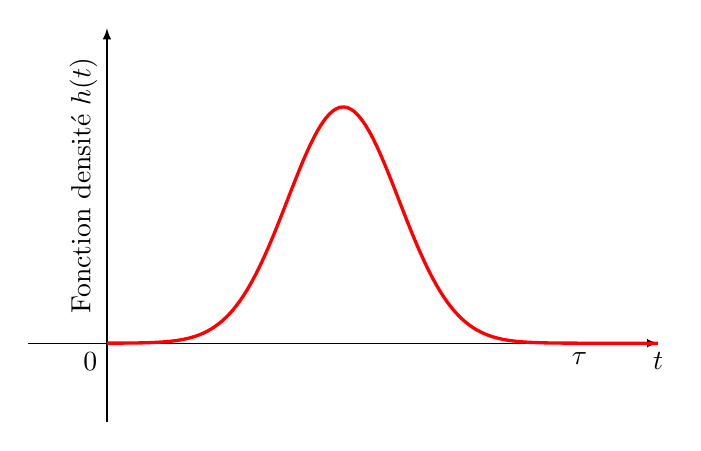
\begin{tikzpicture}
\draw[-latex] (-1,0) -- (7,0) node[below]{$t$};
\draw[-latex] (0,-1) -- (0,0) -- (0,4) node[midway,above,sloped]{Fonction densit\'e $h(t)$};
\draw (6,0) node[below]{$\tau$};
\draw (0,0) node[below left]{0};
\draw[very thick,red,domain=0:7,samples=150] plot(\x,{3*exp(-(\x-3)^2)});
\end{tikzpicture}
\caption{Exemple d'une fonction de densit\'e}
\label{densite}
\end{figure}
On constate que le temps d'incubation de la maladie n'est pas n\'ecessairement le m\^eme pour tous les individus. On peut mod\'eliser cette diversit\'e \`a l'aide d'une fonction positive d'int\'egrale unitaire (dite de densit\'e) $h: [0,\tau] \rightarrow \mathbb{R}_+$ telle que repr\'esent\'ee sur la figure \ref{densite}. On obtient alors le syst\`eme int\'egro-diff\'erentiel:
\[
\left\{ 
\begin{aligned}
\frac{d}{dt}S(t) & =  -rS(t)\int_0^\tau I(t-s)h(s)ds \\
\frac{d}{dt}I(t) & =  rS(t)\int_0^\tau I(t-s)h(s)ds-(a+b)I(t)\\
\frac{d}{dt}R(t) & =  a I(t) \\
\frac{d}{dt}D(t) & =  bI(t)
\end{aligned}
\right. .
\]
On supposera \`a nouveau que pour tout $t \in [-\tau,0]$:
\[
S(t)=0,95,\; I(t)=0,05\, \text{ et } R(t)=D(t)=0.\\  
\]
Pour $j$ entier compris entre 0 et $N$, on pose $t_j=j\times dt$. Pour un pas de temps $dt$ donn\'e, on peut calculer num\'eriquement l'int\'egrale \`a l'instant $t_i$ ($0\leq i \leq N$) \`a l'aide de la m\'ethode des rectangles \`a gauche en utilisant l'approximation:
$$
\int_0^\tau I(t_i-s)h(s)ds \approx dt \times \sum_{j=0}^{p-1}I(t_i-t_j)h(t_j).
$$
\resume{enumerate}
\item On suppose que la fonction $h$ a \'et\'e \'ecrite en Python. Expliquer comment modifier le programme de la question pr\'ec\'edente pour r\'esoudre ce syst\`eme int\'egro-diff\'erentiel (on explicitera les lignes de code n\'ecessaires)
\suspend{enumerate}

\section*{Partie II. Mod\'elisation dans des grilles}

On s'int\'eresse ici \`a une seconde m\'ethode de simulation num\'erique prenant en compte la d\'ependance spatiale de la contagion à l'aide d'une \emph{grille}.\newline
On appelle \emph{grille} de taille $n\times n$ une liste de $n$ listes de longueur $n$, o\`u $n$ est un entier strictement positif.\newline
Chaque case de la grille peut \^etre dans un des quatre \'etats suivants: saine, infect\'ee, r\'etablie, d\'ec\'ed\'ee. On choisit de repr\'esenter ces quatre \'etats par les entiers:
\begin{center}
0 (Sain), 1 (Infect\'e), 2 (R\'etabli) et 3 (D\'ec\'ed\'e)
\end{center} 

L'\'etat des cases d'une grille \'evolue au cours du temps selon des r\`egles simples.\newline
L'\'etat d'une case \`a l'instant $t+1$ ne d\'epend que de son \'etat \`a l'instant $t$ et de l'\'etat de ses huit cases voisines \`a l'instant $t$ (une case du bord n'a que 5 cases voisines et trois pour une case d'un coin). Les \textit{r\`egles de transition} sont les suivantes:
\begin{itemize}
\item une case d\'ec\'ed\'ee reste d\'ec\'ed\'ee,
\item une case infect\'ee devient d\'ec\'ed\'ee avec une probabilit\'e $p_1$ ou r\'etablie avec une probabilit\'e $(1-p_1)$,
\item une case r\'etablie reste r\'etablie,
\item une case saine devient infect\'ee avec une probabilit\'e $p_2$ si elle a au moins une case voisine infect\'ee et reste saine sinon.
\end{itemize}
Initialement, toutes les cases sont dans l'\'etat sain, sauf une, choisie au hasard, qui est dans l'\'etat infect\'e.
\resume{enumerate}
\item Si \texttt{n} désigne un naturel non nul, que renvoie l'instruction Python suivante ?
\begin{lstlisting}
[n*[0] for i in range(n)]
\end{lstlisting}
\suspend{enumerate}
On pourra dans la question suivante utiliser la fonction \texttt{randrange(p)} de la biblioth\`eque \texttt{random} qui, pour un entier positif $p$, renvoie un entier choisi al\'eatoirement entre 0 et $p-1$ inclus.
\resume{enumerate}
\item \'Ecrire en Python une fonction \texttt{init(n)} qui construit une grille $G$ de taille $n\times n$ ne contenant que des cases saines, qui choisit al\'eatoirement une des cases et la transforme en case infect\'ee, et enfin qui renvoie $G$.
\item \'Ecrire en Python une fonction \texttt{compte(G)} qui a pour argument une grille G et renvoie la liste \texttt{[n0,n1,n2,n3]} form\'ee des nombres de cases dans chacun des quatre \'etats. 
\suspend{enumerate}
D'apr\`es les r\`egles de transition, pour savoir si une case saine peut devenir infect\'ee \`a l'instant suivant, il faut d\'eterminer si elle est expos\'ee \`a la maladie, c'est-\`a-dire si elle poss\`ede au moins une case infect\'ee dans son voisinage. 
Pour cela on écrit en Python des fonctions \texttt{voisins(i,j,n)} et \texttt{est\_exposee(G,i,j)}.
\begin{lstlisting}
def voisins(i,j,n):
    V = []
    for a in [-1,0,1]:
        for b in [-1,0,1]:
            u = i + a
            v = j + b
            if # a completer
                V.append([u,v])
    return V
\end{lstlisting}
\begin{lstlisting}
def est_exposee(G,i,j):
    n = len(G)
    V = voisins(i,j,n)
    est_exp = 1
    for v in V:
        est_exp # a completer
    return est_exp == 0
\end{lstlisting}
\resume{enumerate}
\item Quels types de r\'esultats renvoient \texttt{voisins} et \texttt{est\_exposee}?
\item Compl\'eter la ligne 7 de \texttt{voisins} et la ligne 6 de \texttt{est\_exposee}.
\item \'Ecrire une fonction \texttt{suivant(G,p1,p2)} qui fait \'evoluer toutes les cases de la grille G \`a l'aide des r\`egles de transition et renvoie une nouvelle grille correspondant \`a l'instant suivant. Les arguments \texttt{p1} et \texttt{p2} sont les probabilit\'es qui interviennent dans les r\`egles de transition pour les cases infect\'ees et les cases saines. On pourra utiliser la fonction \texttt{bernoulli(p)} suivante qui simule une variable al\'eatoire de Bernoulli de param\`etre $p$: \texttt{bernoulli(p)} vaut 1 avec la probabilit\'e $p$ et 0 avec la probabilit\'e $1-p$.
\begin{lstlisting}
def bernoulli(p):
	x=rd.random()
	if x <=p:
		return 1
	else:
		return 0	
\end{lstlisting}
On reproduit ci-dessous le descriptif de la documentation Python concernant la fonction \texttt{random} de la biblioth\`eque \texttt{random}:

\begin{verbatim}
randomd.random()
    Return the next random floating point number
    in the range [0.0, 1.0)
\end{verbatim}
Avec les r\`egles de transition du mod\`ele utilis\'e, l'\'etat de la grille \'evolue entre les instants $t$ et $t+1$ tant qu'il existe au moins une case infect\'ee.
\item \'Ecrire en Python une fonction \texttt{simulation(n,p1,p2)} qui r\'ealise une simulation compl\`ete avec une grille de taille $n\times n$ pour les probabilit\'es \texttt{p1} et \texttt{p2} et renvoie la liste \texttt{[x0,x1,x2,x3]} form\'ee des proportions de cases dans chacun des quatre \'etats \`a la fin de la simulation (une simulation s'arr\^ete lorsque la grille n'\'evolue plus).
\item Quelle est la valeur de la proportion des cases infect\'ees \texttt{x1} \`a la fin d'une simulation?\\
Quelle relation v\'erifient \texttt{x0,x1,x2} et \texttt{x3}? Comment obtenir \`a l'aide des valeurs de \texttt{x0,x1,x2} et \texttt{x3} la valeur \texttt{x\_atteinte} de la proportion des cases qui ont \'et\'e atteintes par la maladie pendant une simulation?
\suspend{enumerate}

On fixe \texttt{p1} \`a 0,5 et on calcule la moyenne des r\'esultats de plusieurs simulations pour diff\'erentes valeurs de \texttt{p2}. On obtient la courbe de la figure \ref{simu}.


\begin{figure}[!h]
\centering
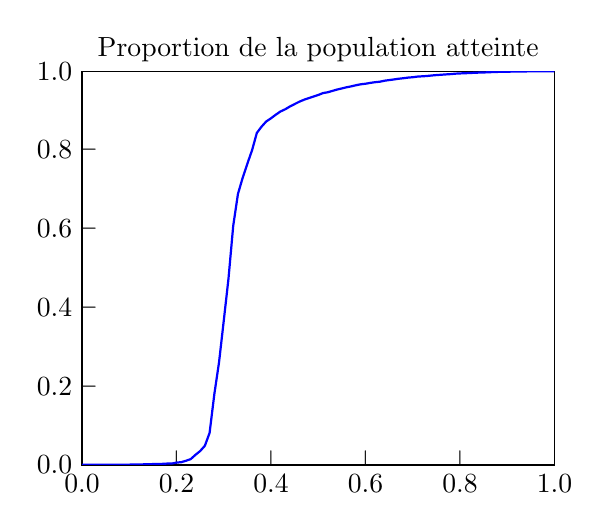
\begin{tikzpicture}[xscale=6,yscale=5]
\draw (0,0) rectangle (1,1);
\draw (.5,1) node[above]{Proportion de la population atteinte};
\foreach \n in {0.0,0.2,0.4,0.6,0.8,1.0}{
\draw (\n,0) node[below]{\n};
\draw (0,\n) node[left]{\n};
}
\clip (0,0) rectangle (1,1);
\foreach \n in {0.2,0.4,0.6,0.8}{
\draw (\n,0) node{$|$};
\draw (0,\n) node[rotate=90]{$|$};
}
\draw[color=blue,thick] (0.0,0.00040) -- (0.01,0.00043) -- (0.02,0.00044) -- (0.03,0.00044) -- (0.04,0.00052) -- (0.05,0.00056) -- (0.06,0.00061) -- (0.07,0.00072) -- (0.08,0.00078) -- (0.09,0.00086) -- (0.1,0.00089) -- (0.11,0.00125) -- (0.12,0.00116) -- (0.13,0.00160) -- (0.14,0.00161) -- (0.15,0.00230) -- (0.16,0.00234) -- (0.17,0.00282) -- (0.18,0.00353) -- (0.19,0.00359) -- (0.2,0.00607) -- (0.21,0.00712) -- (0.22,0.01066) -- (0.23,0.01491) -- (0.24,0.02565) -- (0.25,0.03539) -- (0.26,0.04878) -- (0.27,0.08156) -- (0.28,0.17962) -- (0.29,0.26088) -- (0.3,0.36668) -- (0.31,0.47339) -- (0.32,0.60756) -- (0.33,0.68831) -- (0.34,0.72941) -- (0.35,0.76557) -- (0.36,0.79988) -- (0.37,0.84344) -- (0.38,0.85936) -- (0.39,0.87269) -- (0.4,0.88055) -- (0.41,0.88965) -- (0.42,0.89783) -- (0.43,0.90341) -- (0.44,0.91054) -- (0.45,0.91668) -- (0.46,0.92274) -- (0.47,0.92776) -- (0.48,0.93185) -- (0.49,0.93592) -- (0.5,0.93976) -- (0.51,0.94463) -- (0.52,0.94662) -- (0.53,0.95016) -- (0.54,0.95362) -- (0.55,0.95642) -- (0.56,0.95937) -- (0.57,0.96174) -- (0.58,0.96459) -- (0.59,0.96696) -- (0.6,0.96832) -- (0.61,0.97047) -- (0.62,0.97223) -- (0.63,0.97339) -- (0.64,0.97597) -- (0.65,0.97763) -- (0.66,0.97920) -- (0.67,0.98102) -- (0.68,0.98233) -- (0.69,0.98390) -- (0.7,0.98486) -- (0.71,0.98648) -- (0.72,0.98718) -- (0.73,0.98797) -- (0.74,0.98927) -- (0.75,0.99037) -- (0.76,0.99112) -- (0.77,0.99203) -- (0.78,0.99275) -- (0.79,0.99388) -- (0.8,0.99451) -- (0.81,0.99502) -- (0.82,0.99553) -- (0.83,0.99608) -- (0.84,0.99664) -- (0.85,0.99693) -- (0.86,0.99752) -- (0.87,0.99797) -- (0.88,0.99841) -- (0.89,0.99856) -- (0.9,0.99895) -- (0.91,0.99910) -- (0.92,0.99932) -- (0.93,0.99952) -- (0.94,0.99967) -- (0.95,0.99980) -- (0.96,0.99990) -- (0.97,0.99993) -- (0.98,1.00000) -- (0.99,1.00000) -- (1.0,1.00000);
\end{tikzpicture}
\caption{Repr\'esentation de la proportion de la population qui a \'et\'e atteinte par la maladie pendant la simulation en fonction de la probabilit\'e $p2$}
\label{simu}
\end{figure}
\resume{enumerate}
\item On appelle \textit{seuil critique de pand\'emie} la valeur de \texttt{p2} \`a partir de laquelle plus de la moiti\'e de la population a \'et\'e atteinte par la maladie \`a la fin de la simulation. On suppose que les valeurs de \texttt{p2} et \texttt{x\_atteinte} utilis\'ees pour tracer la courbe de la figure \ref{simu} on \'et\'e stock\'ees dans deux listes de m\^eme longueur \texttt{Lp2} et \texttt{Lxa}.\newline
\'Ecrire en Python une fonction \texttt{seuil(Lp2,Lxa)} qui d\'etermine par dichotomie un encadrement \texttt{[p2cmin,p2cmax]} du seuil critique de pand\'emie avec la plus grande pr\'ecision possible. On supposera que la liste \texttt{Lp2} cro\^\i t de 0 \`a 1 et que la liste \texttt{Lxa} des valeurs correspondantes est croissante.
\suspend{enumerate}
Pour \'etudier l'effet d'une campagne de vaccination, on immunise au hasard \`a l'instant initial une fraction \texttt{q} de la population. On a \'ecrit la fonction \texttt{init\_vac(n,q)}.
\begin{lstlisting}
def init_vac(n,q):
	G = init(n)
	nvac = int(q*n**2)
	k = 0
	while k < nvac:
		i = rd.randrange(n)
		j = rd.randrange(n)
		if G[i][j] == 0:
			G[i][j] = 2
			k += 1
	return G
\end{lstlisting}
\resume{enumerate}
\item Peut-on supprimer le test en ligne 8?
\item Que renvoie l'appel \texttt{init\_vac(5,0.2)}?
\end{enumerate}
